\documentclass[solutionorbox,answers]{exam} %,answers

%%%%%%%%%%%%%%%%%%%%%%%%%%%%%%%%%%%%%%%%%%%%%%%%%%%%%%%%%%%%%%%
% Update to change header
\newcommand{\courseName}{CS 577}
\newcommand{\assignmentName}{Assignment 9 -- Network Flow}
\newcommand{\semester}{Fall 2022}
%%%%%%%%%%%%%%%%%%%%%%%%%%%%%%%%%%%%%%%%%%%%%%%%%%%%%%%%%%%%%%%

\usepackage[utf8]{inputenc}
\usepackage[T1]{fontenc}

\usepackage{amsmath}
\usepackage{amsfonts}
\usepackage{amsthm}
\usepackage{booktabs}
\usepackage{tkz-graph}
\usepackage[ruled]{algorithm2e}
\usepackage{graphicx}
%\usepackage{wrapfig}

\usepackage{hyperref}

\pagestyle{headandfoot}
\runningheadrule
\firstpageheader{\courseName}{\huge \assignmentName}{\semester}
\runningheader{\courseName}
{\assignmentName}
{\semester}
\firstpagefooter{}{}{}
\runningfooter{}{Page \thepage\ of \numpages}{}

\begin{document}

\begin{center}
\fbox{\parbox{5.5in}{\centering
Answer the questions in the boxes provided on the
question sheets. If you run out of room for an answer,
add a page to the end of the document. \\
\vspace{0.1in}
}}
\end{center}
\vspace{0.1in}
\makebox[0.48\textwidth]{Name:\enspace\hrulefill} \qquad
\makebox[0.48\textwidth]{Wisc id:\enspace\hrulefill}

\begin{questions}

\section*{Network Flow}

\question
\emph{Kleinberg, Jon. Algorithm Design (p. 415, q. 3a)}
The figure below shows a flow network on which an $s-t$ flow has been computed. The capacity of each edge appears as a label next to the edge, and the flow is shown in boxes next to each edge. An edge with no box has no flow being sent down it.
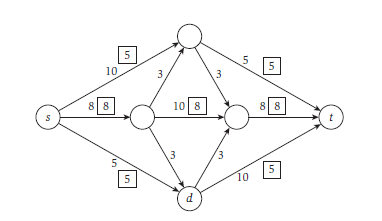
\includegraphics[width=0.6\linewidth]{FlowGraph.png}
\begin{parts}
\part What is the value of this flow?
\begin{solutionbox}{0.5in}

\end{solutionbox}

\part Please draw the \textbf{residual graph} associated with this flow.
\begin{solutionbox}{2in}

\end{solutionbox}


\part Is this a maximum $s-t$ flow in this graph? If not, describe an augmenting path that would increase the total flow.
\begin{solutionbox}{0.5in}

\end{solutionbox}
\end{parts}

\newpage

\question
\emph{Kleinberg, Jon. Algorithm Design (p. 419, q. 10)}
Suppose you are given a directed graph $G=(V,E)$. This graph has a positive integer capacity $c_e$ on each edge, a source $s\in V$, a sink $t\in V$. You are also given a maximum $s-t$ flow through $G$: $f$. You know that this flow is \emph{acyclic} (no cycles with positive flow all the way around the cycle), and every flow $f_e\in f$ has an integer value.

Now suppose we pick an edge $e^*$ and reduce its capacity by 1 unit. Show how to find a maximum flow in the resulting graph $G^*$ in time $O(m+n)$, where $n=|V|$ and $m=|E|$.
\begin{solutionbox}{2in}


\end{solutionbox}

\question
\emph{Kleinberg, Jon. Algorithm Design (p. 420, q. 11)}
A friend of yours has written a very fast piece of code to calculate the maximum flow based on repeatedly finding augmenting paths. However, you realize that it's not always finding the maximum flow. Your friend never wrote the part of the algorithm that uses backward edges! So their program finds only augmenting paths that include all forward edges, and halts when no more such augmenting paths remain. (Note: We haven't specified \emph{how} the algorithm selects forward-only augmenting paths.)

When confronted, your friend claims that their algorithm may not produce the maximum flow every time, but it is guaranteed to produce flow which is within a factor of $b$ of maximum. That is, there is some constant $b$ such that no matter what input you come up with, their algorithm will produce flow at least $1/b$ times the maximum possible on that input.

Is your friend right? Provide a proof supporting your choice.
\begin{solutionbox}{3in}


\end{solutionbox}

\newpage

\question
\emph{Kleinberg, Jon. Algorithm Design (p. 418, q. 8)}
Consider this problem faced by a hospital that is trying to evaluate whether its blood supply is sufficient:

In a (simplified) model, the patients each have blood of one of four types: A, B, AB, or O. Blood type A has the A antigen, type B has the B antigen, AB has both, and O has neither. Patients with blood type A can receive either A or O blood. Likewise patients with type B can receive either B or O type blood. Patients with type O can only receive type O blood, and patients with type AB can receive any of the four types.

\begin{parts}
\part Let integers $s_O, s_A, s_B, s_{AB}$ denote the hospital's blood supply on hand, and let integers $d_A, d_B, d_O, d_{AB}$ denote their projected demand for the coming week. Give a polynomial time algorithm to evaluate whether the blood supply is enough to cover the projected need.
\begin{solutionbox}{3.25in}


\end{solutionbox}

\part Network flow is one of the most powerful and versatile tools in the algorithms toolbox, but it can be difficult to explain to people who don't know algorithms. Consider the following instance. Show that the supply is \textbf{insufficient} in this case, and provide an explanation for this fact that would be understandable to a non-computer scientist. (For example: to a hospital administrator.) Your explanation should not involve the words \emph{flow}, \emph{cut}, or \emph{graph}.

\begin{tabular}{lll}
blood type & supply & demand \\
\hline
O & 50 & 45 \\
A & 36 & 42 \\
B & 11 & 8 \\
AB & 8 & 3
\end{tabular}

\begin{solutionbox}{1.75in}


\end{solutionbox}

\end{parts}

\newpage

\question Implement the Ford-Fulkerson method for finding maximum flow in graphs with only integer edge capacities, in either C, C++, C\#, Java, or Python. Be efficient and implement it in $O(mF)$ time, where $m$ is the number of edges in the graph and $F$ is the value of the maximum flow in the graph. We suggest using BFS or DFS to find augmenting paths. (You may be able to do better than this.)

The input will start with a positive integer, giving the number of instances that follow. For each instance, there will be two positive integers, indicating the number of nodes $n = |V|$ in the graph and the number of edges $|E|$ in the graph. Following this, there will be $|E|$ additional lines describing the edges. Each edge line consists of a number indicating the source node, a number indicating the destination node, and a capacity. The nodes are not listed separately, but are numbered $\{1\ldots n\}$.

Your program should compute the maximum flow value from node 1 to node $n$ in each given graph.

A sample input is the following:

\begin{verbatim}
2
3 2
2 3 4
1 2 5
6 9
1 2 9
1 3 4
2 4 1
2 5 6
3 4 4
3 5 5
4 6 8
5 6 5
5 6 3
\end{verbatim}

The sample input has two instances. For each instance, your program should output the maximum flow on a separate line. Each output line should be terminated by a newline. The correct output for the sample input would be:
\begin{verbatim}
4
11
\end{verbatim}

\end{questions}

\end{document}
